% LaTeX source for PyMS User Guide

\documentclass[twoside,a4paper]{book}

\usepackage{epsfig}
\usepackage{graphicx}
\usepackage{makeidx}
\usepackage{tlk2e/tlk2e}
\usepackage{url}

\setlength{\topmargin}{0.0cm}
\setlength{\evensidemargin}{0.0cm}
\setlength{\oddsidemargin}{0.0cm}
\setlength{\textwidth}{16.0cm}
\setlength{\textheight}{23.0cm}
%\setlength{\footskip}{0.0cm}

\parskip 0.2cm
\parindent 0cm
\makeindex

\begin{document}

\frontmatter

\title{
\includegraphics{logo/PyMS.eps}
\Large{PyMS2 User Guide}}
\author{Andrew Isaac and Vladimir Liki\'{c}\\
with contributions from:\\
\medskip}

\medskip

\version{PyMS version 1.0}

\abstract{A Python toolkit for processing of chromatography--mass spectrometry
data}

\maketitle
\tableofcontents

\input epsf

\newpage

\setcounter{chapter}{1}
\setcounter{section}{0}
\pagenumbering{arabic}
% chapter01.tex

 %%%%%%%%%%%%%%%%%%%%%%%%%%%%%%%%%%%%%%%%%%%%%%%%%%%%%%%%%%%%%%%%%%%%%%%%%%%%%
 %                                                                           %
 %    PyMS documentation                                                     %
 %    Copyright (C) 2005-8 Vladimir Likic                                    %
 %                                                                           %
 %    The files in this directory provided under the Creative Commons        %
 %    Attribution-NonCommercial-NoDerivs 2.1 Australia license               %
 %    http://creativecommons.org/licenses/by-nc-nd/2.1/au/                   %
 %    See the file license.txt                                               %
 %                                                                           %
 %%%%%%%%%%%%%%%%%%%%%%%%%%%%%%%%%%%%%%%%%%%%%%%%%%%%%%%%%%%%%%%%%%%%%%%%%%%%%

\chapter{Introduction}

\section{About PyMS}

PyMS is a Python toolkit for processing of chromatography--mass spectrometry
data. The main idea behind PyMS is to provide a framework and a set of
components for rapid development and testing of methods for processing of
chromatography--mass spectrometry data. An important objective of PyMS is
to decouple processing methods form visualization and the concept of
interactive processing. This is useful for high-throughput processing tasks
and when there is a need to run calculations in the batch mode.

PyMS is modular and consists of several sub-packages written in Python
programming language \cite{python}. PyMS is released as open source,
under the GNU Public License version 2.

There are four parts of the pyms project:

\begin{itemize}
  \item pyms -- The PyMS code
  \item pyms-docs -- The PyMS documentation
  \item pyms-test -- Examples of PyMS use
\end{itemize}

Each part is a separate project on Google Code that can be downloaded
separately. The data used in PyMS documentation and examples is available
from the Bio21 Institute server:\\
{\tt http://bioinformatics.bio21.unimelb.edu.au/pyms-data/}\\
In addition, the current PyMS API documentation is available from here:\\
{\tt http://bioinformatics.bio21.unimelb.edu.au/pyms.api/index.html}

\section{PyMS installation}

There are several ways to install PyMS depending your computer configuration
and preferences. The recommended way install PyMS is to compile Python
from sources and install PyMS within the local Python installation. This
procedure is described below.

PyMS has been developed on Linux, and a detailed installation instructions
for Linux are given below. Installation on any Unix-like system should be
similar. We have not tested PyMS under Microsoft Windows.

\subsection{Downloading PyMS source code}

PyMS source code resides on Google Code servers, and can be accessed
from the following URL: http://code.google.com/p/pyms/. Under the
section "Source" one can find the instructions for downloading the
source code. The same page provides the link under "This project's
Subversion repository can be viewed in your web browser" which allows
one to browse the source code on the server without actually downloading
it.

Google Code maintains the source code with the program `subversion'
(an open-source version control system). To download the source code
one needs to use the subversion client program called `svn'. The `svn'
client exists for all mainstream operating systems\footnote{For example,
on Linux CentOS 4 we have installed the RPM package
`subversion-1.3.2-1.rhel4.i386.rpm' to provide us with the subversion
client `svn'.}, for more information see http://subversion.tigris.org/.
The book about subversion is freely available on-line at
http://svnbook.red-bean.com/. Subversion has extensive functionality.
However only the very basic functionality is needed to download PyMS
source code.

If the computer is connected to the internet and the subversion client
is installed, the following command will download the latest PyMS source
code:

\begin{verbatim}
$ svn checkout http://pyms.googlecode.com/svn/trunk/ pyms
A    pyms/Peak
A    pyms/Peak/__init__.py
A    pyms/Peak/List
A    pyms/Peak/List/__init__.py
.....
Checked out revision 71.
\end{verbatim}

\subsection{PyMS installation}

PyMS installation consists of placing the PyMS code directory (pyms/) in
place visible to Python interpreter.  This can be in the standard place
for 3rd party software (the directory site-packages/). If PyMS code is
placed in a non-standard place the Python interpreter needs to be made
aware of it before before it is possible to import PyMS modules (see the
Python sys.path.append() command).

We recommend compiling your own Python installation for PyMS.

In addition to the PyMS core source code, a number of external packages
is used to provide additional functionality. These are explained below.

\subsection{\label{subsec:numpy}Package `NumPy'}

The package NumPy is provides numerical capabilities to Python. This
package is used throughout PyMS (and also required for some external
packages used in PyMS), to its installation is mandatory.

The NumPy web site {\tt http://numpy.scipy.org/} provides the installation
instructions and the link to the source code.

\subsection{\label{subsec:pycdf}Package `pycdf' (required for reading
ANDI-MS files)}

The pycdf (a python interface to Unidata netCDF library) source and
installation instructions can be downloaded from\\
{\tt http://pysclint.sourceforge.net/pycdf/}. Follow the installation
instructions to install pycdf.

\subsection{\label{subsec:pycluster}Package `Pycluster' (required for peak
alignment by dynamic programming)}

The peak alignment by dynamic programming is located in the subpackage
pyms.Peak.List.DPA. This subpackage used the Python package `Pycluster'
as the clustering engine. Pycluster with its installation instructions
can be found here:\\
{\tt http://bonsai.ims.u-tokyo.ac.jp/~mdehoon/software/cluster/index.html}.

\subsection{\label{subsec:scipy-ndmage}Package `scipy.ndimage' (required
for TopHat baseline corrector)}

If the full SciPy package is installed the `ndimage' will be available. However
the SciPy contains large amount of functionality, and its installation is
somewhat involved. In some situations in may be preferable to install only
the subpackage `ndimage'. The UrbanSim web site \cite{urbansim} provides
instructions how to install a local copy of `ndimage'. These instructions
and the link to the file `ndimage.zip' are here:\\
{\tt http://www.urbansim.org/opus/releases/opus-4-1-1/docs/installation/scipy.html}

\subsection{\label{subsec:matplotlib}Package 'matplotlib' (required 
for plotting information in Display module)}

The displaying of information such as Ion Chromatograms and detected peaks
is done using the package matplotlib. The matplotlib package and user information
can be accessed at:\\
{\tt http://matplotlib.sourceforge.net/}

\section{Current PyMS development environment}

PyMS is currently being developed with the following packages:

\begin{verbatim}
Python-2.5.2
numpy-1.1.1
netcdf-4.0
pycdf-0.6-3b
Pycluster-1.41
matplotlib-0.99.1.2
\end{verbatim}

A quick installation guide for packages required by PyMS is given below.

\begin{enumerate}

\item Python installation:

\begin{verbatim}
$ tar xvfz Python-2.5.2.tgz
$ cd Python-2.5.2
$ ./configure
$ make
$ make install
\end{verbatim}

\noindent
This installs python in /usr/local/lib/python2.5.  Make sure that python called
from the command line is the one just compiled and installed.

\item NumPy installation:

\begin{verbatim}
$ tar xvfz numpy-1.1.1.tar.gz
$ cd numpy-1.1.1
$ python setup.py install
\end{verbatim}

\item pycdf installation

Pycdf has two dependencies: the Unidata netcdf library and NumPy. The NumPy
installation is described above. To install pycdf, the netcdf library must
be downloaded\\
({\tt http://www.unidata.ucar.edu/software/netcdf/index.html}),\\
compiled and installed first:

\begin{verbatim}
$ tar xvfz netcdf.tar.gz
$ cd netcdf-4.0
$ ./configure
$ make
$ make install
\end{verbatim}

The last step will create several binary `libnetcdf*' files in /usr/local/lib.
pycdf can be installed as follows:

\begin{verbatim}
$ tar xvfz pycdf-0.6-3b
$ cd pycdf-0.6-3b
$ python setup.py install
\end{verbatim}

\item Pycluster installation

\begin{verbatim}
$ tar xvfz Pycluster-1.42.tar.gz
$ cd Pycluster-1.42
$ python setup.py install
\end{verbatim}

\item ndimage installation:

\begin{verbatim}
$ unzip ndimage.zip
$ cd ndimage
$ python setup.py install --prefix=/usr/local
\end{verbatim}

\noindent
Since ndimage was installed outside the scipy package, this requires some manual
correction:

\begin{verbatim}
$ cd /usr/local/lib/python2.5/site-packages
$ mkdir scipy
$ touch scipy/__init__.py
$ mv ndimage scipy
\end{verbatim}

\item matplotlib installation:

\begin{verbatim}
$ tar xvfz matplotlib-0.99.1.2
$ cd matplotlib-0.99.1.1
$ python setup.py build
$ python setup.py install
\end{verbatim}

\noindent
The pyms.Display package uses the TKAgg backend for matplotlib. As this is
not the default backend, the matplotlibrc file must be edited. To locate the
matplotlibrc file, in a python interactive session:

\begin{verbatim}
>>> import matplotlib
>>> matplotlib.matplotlib_fname()
\end{verbatim}

\noindent
Open the matplotlibrc file in a text editor and adjust the 'backend'
parameter to 'TKAgg'.

\end{enumerate}

\section{Troubleshooting}

The PyMS is essentially a python library (a `package' in python parlance, which
consists of several `sub-packages'), which for some functionality depends on
other python libraries, such as NumPy, pycdf, and Pycluster. The most likely
problem with PyMS installation is a problem with installing one of the PyMS
dependencies.

\subsection{Pycdf import error}

On Red Hat Linux 5 the SELinux is enabled by default, and this causes the
following error while trying to import properly installed pycdf:

\begin{verbatim}
$ python
Python 2.5.2 (r252:60911, Nov  5 2008, 16:25:39)
[GCC 4.1.1 20070105 (Red Hat 4.1.1-52)] on linux2
Type "help", "copyright", "credits" or "license" for more information.
>>> import pycdf
Traceback (most recent call last):
  File "<stdin>", line 1, in <module>
  File "/usr/local/lib/python2.5/site-packages/pycdf/__init__.py", line 22, in <module>
    from pycdf import *
  File "/usr/local/lib/python2.5/site-packages/pycdf/pycdf.py", line 1096, in <module>
    import pycdfext as _C
  File "/usr/local/lib/python2.5/site-packages/pycdf/pycdfext.py", line 5, in <module>
    import _pycdfext
ImportError: /usr/local/lib/python2.5/site-packages/pycdf/_pycdfext.so:
    cannot restore segment prot after reloc: Permission denied
\end{verbatim}

This problem is removed simply by disabling SELinux (login as `root', open the
menu Administration $\rightarrow$ Security Level and Firewall, tab SELinux,
change settings from `Enforcing' to `Disabled').

This problem is likely to occur on Red Hat Linux derivative distributions such
as CentOS.

\section{PyMS tutorial and examples}

A tutorial illustrating various PyMS features in provided in subsequent chapter
of this User Guide. The commands executed interactively are grouped together
by example, and provided as Python scripts in the project `pyms-test' (this is
a Google code project, similar to the project `pyms' which contains the PyMS
source code).

The setup used in the examples below is as follows. The projects `pyms',
`pyms-test', `pyms-docs', and `data' are all in the same directory,
`/x/PyMS'. In the project `pyms-test' there is a directory corresponding to
each example coded with the example number (ie. {\tt pyms-test/21a/}
corresponds to Example 1a in Chapter 2).

In each example directory, there is a script named `proc.py' which contains
the commands given in the example.  Provided that the paths to `pyms' and
`pyms-data' are set properly, these scripts could be run with the following
command:

\begin{verbatim}
$ python proc.py
\end{verbatim}

Before running each example the Python interpreter was made aware of the
PyMS location with the following commands:

\begin{verbatim}
import sys
sys.path.append("/x/PyMS")
\end{verbatim}

For brevity these commands will not be shown in the examples below, but
they are included in `pyms-test' example scripts.  The above path may need
to be adjusted to match your own directory structure.

All data files (raw data files, peak lists etc.) used in the example below
can be found at \\
{\tt http://bioinformatics.bio21.unimelb.edu.au/pyms/data/} \\
and are assumed to be located in the `data' directory.




% chapter02.tex

 %%%%%%%%%%%%%%%%%%%%%%%%%%%%%%%%%%%%%%%%%%%%%%%%%%%%%%%%%%%%%%%%%%%%%%%%%%%%%
 %                                                                           %
 %    PyMS documentation                                                     %
 %    Copyright (C) 2005-8 Vladimir Likic                                    %
 %                                                                           %
 %    The files in this directory provided under the Creative Commons        %
 %    Attribution-NonCommercial-NoDerivs 2.1 Australia license               %
 %    http://creativecommons.org/licenses/by-nc-nd/2.1/au/                   %
 %    See the file license.txt                                               %
 %                                                                           %
 %%%%%%%%%%%%%%%%%%%%%%%%%%%%%%%%%%%%%%%%%%%%%%%%%%%%%%%%%%%%%%%%%%%%%%%%%%%%%

\chapter{Using PyMS}

\section{Introduction}

The setup used for the examples below is as follows. The projects 'pyms',
'pyms-test', 'pyms-docs', and 'pyms-data' were downloaded in the directory
{\tt /home/current/proj/PyMS}. In the project 'pyms-test' there is a directory
corresponding to each example coded with the example number (ie.
{\tt pyms-test/01/} corresponds to Example 1). In each example directory
there is a script named 'proc.py' which contains the commands given in
the example. Provided that the paths to 'pyms' and 'pyms-data' are set
properly, these scripts could be run by simply:

\$ python proc.py

Before running each example the Python interpreter was made aware of the
PyMS location with the following commands:

\begin{verbatim}
import sys
sys.path.append("/home/current/proj/PyMS/")
\end{verbatim}

For brevity these commands will not be shown in the examples below, but
they are included in 'pyms-test' example scripts.  The above path need
to be adjusted to match your own location of pyms.

All data files (raw data files, peak lists etc) used in the example below
can be found in 'pyms-data'.


\section{Example 1: Reading of GC-MS data and basic manipulations with
data}

\subsection{Reading ChemStation GC-MS data into PyMS}

\noindent
{\em The python script for this example is pyms-test/01/proc.py}

The PyMS package pyms.IO provides capabilities to read the raw GC-MS
data stored in the ANDI-MS format. The function IO.ANDI.ChemStation()
provides the interface to ANDI-MS data files saved from Agilent
ChemStation software.\footnote{ANDI-MS data format stands for Analytical
Data Interchange for Mass Spectrometry, and was developed for the
description of mass spectrometric data developed in 1994 by Analytical
Instrument Association. ANDI-MS is essentially a recommendation, and
it is up to individual vendors of mass spectrometry processing software
to implement "export to ANDI-MS" feature in their software.}

The file '0510\_217.CDF' is a GC-MS experiment exported from Agilent
ChemStation (located in 'pyms-data'). This file can be loaded in the
memory as follows:

\begin{verbatim}
>>> from pyms.IO.ANDI.Class import ChemStation
>>> andi_file = "/home/current/proj/PyMS/pyms-data/0510_217.CDF"
>>> andi_data = ChemStation(andi_file)
 -> Processing netCDF file '/home/current/proj/PyMS/pyms-data/0510_217.CDF'
    [ 2784 scans, masses from 50 to 550 ]
>>>
\end{verbatim}

\noindent
The above command creates the object 'andi\_data' which is an {\em instance}
of the class IO.ANDI.ChemStation.

\subsection{Exploring an ANDI-MS data object}

\noindent
{\em The python script for this example is pyms-test/01/proc.py}

The object 'andi\_data' has several attributes and methods associated with it.

\begin{verbatim}
>>> print "ANDI-MS data filename:", andi_data.get_filename()
ANDI-MS data filename: /home/current/proj/PyMS/pyms-data/0510_217.CDF
\end{verbatim}

The method {\tt get\_tic()} return total ion chromatogram (TIC) of the data
as an IonChromatogram object:

\begin{verbatim}
tic = andi_data.get_tic()
\end{verbatim}

\noindent
An IonChromatogram object is a one dimensional vector containing
mass intensities as a function of retention time. This can can be either
m/z channel intensities (for example, ion chromatograms at m/z = 65),
or cumulative intensities over all measured m/z (TIC).

The method {\tt get\_ic\_at\_index(i)} returns i-th ion chromatogram, as
an IonChromatogram object. For example, to get the first ion chromatogram
from the data:

\begin{verbatim}
ic = andi_data.get_ic_at_index(1)
\end{verbatim}

The method {\tt get\_ic\_at\_mass(MZ)} returns the ion chromatogram for
m/z = MZ.  For example, to get the ion chromatogram that corresponds
to m/z = 73:

An ion chromatogram object has a method {\tt is\_tic()} which returns
True is the ion chromatogram is TIC, False otherwise:

\begin{verbatim}
>>> print "'tic' is a TIC:", tic.is_tic()
'tic' is a TIC: True
>>> print "'ic' is a TIC:",ic.is_tic()
'ic' is a TIC: False
\end{verbatim}

\subsection{Writing data to a file}

\noindent
{\em The python script for this example is pyms-test/01/proc.py}

The method {\tt write()} of IonChromatogram object allows one to save
the ion chromatogram object to a file:

\begin{verbatim}
>>> tic.write("output/tic.dat")
>>> ic.write("output/ic.dat")
\end{verbatim}

The method {\tt get\_intensity\_matrix()} of ChemStation object returns
the entire matrix of intensities:

\begin{verbatim}
>>> im = andi_data.get_intensity_matrix()
>>> print "Dimensions of the intensity matrix are:",len(im),"x",len(im[0])
Dimensions of the intensity matrix are: 2784 x 501
\end{verbatim}

\noindent
This data matrix contains 2784 time points (MS scans), and each time point
corresponds to a mass spectrum of 501 m/z points.

The intensity matrix can be saved to a file with the function 'save\_data()':

\begin{verbatim}
save_data("output/im.dat", im)
\end{verbatim}

The entire data (ie. ChemStation object) can be saved as CSV with the method
{\tt export\_csv()}. For example,

\begin{verbatim}
>>> andi_data.export_csv("output/data")
\end{verbatim}

\noindent
will create 'data.im.csv, data.mz.csv, and data.rt.csv where these are the
intensity matrix, retention time vector, and m/z vector in the CSV format.

\subsection{Using Octave or Matlab to plot the data}

The ion chromatogram object saved with with the {\tt write{}} method is a
plain ASCII file which contains a pair of (retention time, intensity) per
line:

\begin{verbatim}
$ cat tic.dat
 305.666      745997
 306.009      726566
 306.352      717704
 306.695      684214
 307.038      701866
 307.381      893306
 307.724     1278099
 308.067     1290984
 308.410      925558
 308.752      644122
[..output deleted..]
\end{verbatim}

\noindent
The left column is the retention time in seconds, while the right column
is the corresponding intensity. This data can be conveniently loaded and
plotted in matlab or octave:

\begin{verbatim}
octave:1> load tic.dat
octave:2> plot(tic(:,1)/60, tic(:,2))
\end{verbatim}

The output is shown in Figure \ref{ticplot}. In the above command the
time was divided by 60 to convert the x-axis into minutes.

\begin{figure}[htp]
\begin{center}
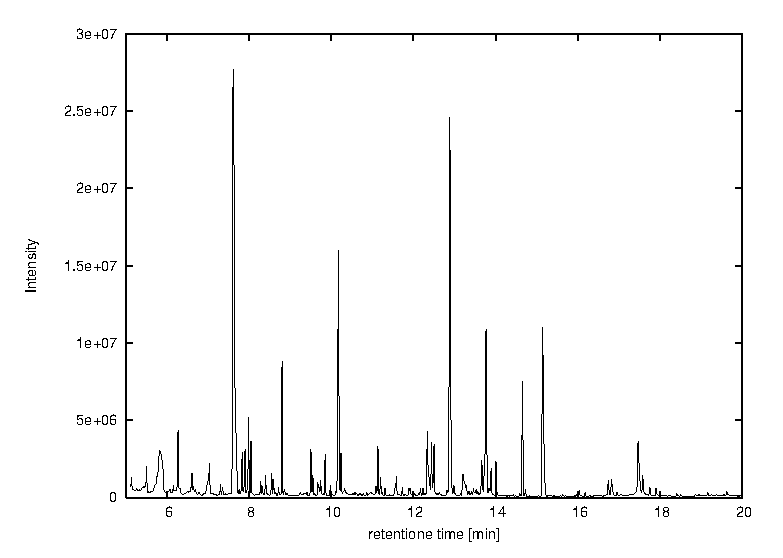
\includegraphics{graphics/tic.eps}
\caption{The octave plot of the file 'tic.dat'.}
\label{ticplot}
\end{center}
\end{figure}

\section{Example 2: Creating signal peaks}

\noindent
{\em The python script for this example is pyms-test/02/proc1.py}

In PyMS a signal peak is represented as 'Peak' object defined in
pyms.Peak.Class.py. A peak object is initialized with two arguments:
peak retention time and peak raw area. The following commands create
a peak named 'p' with the retetion time of 5.553 min and a peak area
of 2759280 (this is the peak no. 3 in the ChemStation peak area report
file 'a0806\_140.txt'):

\begin{verbatim}
>>> from pyms.Peak.Class import Peak
>>> p = Peak(5.553*60.0,2759280)
\end{verbatim}

\noindent
As a matter of convention PyMS internally stores retention times in
seconds, hence above the retention time is multiplied by 60. Peak
raw area is in arbitrary units.

Peak properties can be accessed through its attributes:

\begin{verbatim}
>>> print "Peak retention time is", p.rt
Peak retention time is 333.18
>>> print "Peak raw area is", p.raw_area
Peak raw area is 2759280.0
\end{verbatim}

\noindent
Other important properties of a peak object are peak normalized area
and peak mass spectrum. The peak created in the above example does
not have values associated with these two attributes, and they are
merely initialized to 'None':

\begin{verbatim}
>>> print "Peak normalized area is", p.norm_area
Peak normalized area is None
>>> print "Peak mass spectrum is", p.mass_spectrum
Peak mass spectrum is None
\end{verbatim}

\noindent
The peak mass spectrum can be set by calling the method {\tt set\_mass\_spectrum()}.
This method requires the raw data, and fetches mass spectrum at peak
retention time:

\begin{verbatim}
>>> p.set_mass_spectrum(andi_data)
\end{verbatim}

\noindent
This will set the mass spectrum attribute: 

\begin{verbatim}
>>> print p.mass_spectrum
 49976  54520 102752  15570   1872  18392   8765  14966  46136  16141
  1635   1743    686   1019    712   1199   1641   3182   1234  30400
  4261   3746   3348  82392   8354  24824   3797   6086  23312 140480
[--output deleted--]
\end{verbatim}

\noindent
These are m/z channel intensities in arbitrary units. The m/z values
themselves are in the mass list attribute:

\begin{verbatim}
>>> print p.mass_list
[50, 51, 52, 53, 54, 55, 56, 57, 58, 59, 60, 61, 62, 63, 64, 65,
66, 67, 68, 69, 70, 71, 72, 73, 74, 75, 76, 77, 78, 79, 80, 81,
[--outout deleted--]
\end{verbatim}

\noindent
The length of the two arrays must match:

\begin{verbatim}
>>> print len(p.mass_spectrum)
501
>>> print len(p.mass_list)
501
\end{verbatim}

The mass spectrum can be written to a file by calling the peak
{\tt write_mass_spectum()} method:

\begin{verbatim}
>>> p.write_mass_spectrum("output/ms.dat")
\end{verbatim}

\noindent
The file 'output/ms.dat' contains the pairs (mz, intensity), one pair
per line:

\begin{verbatim}
$ head output/ms.dat
  50.000        49976.000
  51.000        54520.000
  52.000       102752.000
  53.000        15570.000
  54.000         1872.000
  55.000        18392.000
  56.000         8765.000
  57.000        14966.000
  58.000        46136.000
  59.000        16141.000
\end{verbatim}

\noindent
From this file the mass spectrum can be easily visualized in gnuplot:

\begin{verbatim}
gnuplot> plot "ms.dat" with impulses
\end{verbatim}




\bibliography{bibtex/refbase}
\bibliographystyle{unsrt}

\backmatter
\printindex

\end{document}

